\documentclass[crop,tikz,pgf]{standalone}

\usetikzlibrary{arrows,automata,positioning}

\begin{document}
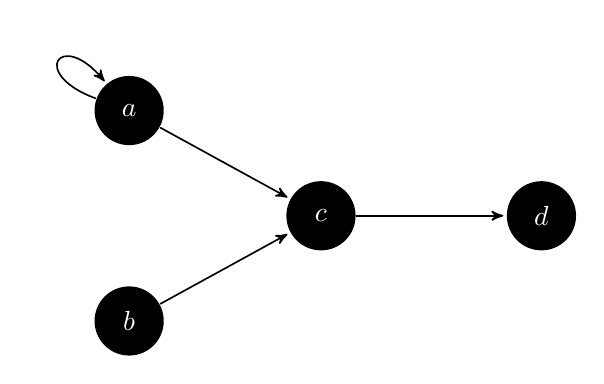
\begin{tikzpicture}[->,>=stealth',shorten >=1pt,auto,node distance=2.8cm,semithick]
	\tikzstyle{every state}=[fill=black,draw=none,text=white]

	\node[state] (C) {$c$};
	\node[state] (A) [above left = 0.7 and 1.8 of C] {$a$};
	\node[state] (B) [below left = 0.7 and 1.8 of C] {$b$};
	\node[state] (D) [right of = C] {$d$};

	\path (A) edge (C);
        \path (B) edge (C);
        \path (C) edge (D);
        \draw (A) to [out=160,in=130,looseness=10] (A);
\end{tikzpicture}
\end{document}